\documentclass[a4paper,14pt]{extarticle}

\usepackage[left=30mm, right=10mm, top=20mm, bottom=20mm]{geometry}

\usepackage[T2A]{fontenc}
\usepackage[utf8]{inputenc}
\usepackage[russian]{babel}
\usepackage{tempora}
\usepackage{type1cm}
\usepackage{indentfirst}

\usepackage{minted}
\usepackage{xcolor}

\usepackage{siunitx}
\usepackage{booktabs}
\usepackage{multirow}


\usepackage{csquotes}
\usepackage[
    parentracker=true,
    backend=biber,
    style=gost-numeric,
    sorting=nty
]{biblatex}

\usepackage[nodisplayskipstretch]{setspace}
\usepackage[none]{hyphenat}
\usepackage{fancyhdr}
\usepackage{titlesec}
\usepackage{tocloft}

\usepackage{amssymb}
\usepackage{amsmath}
\usepackage{tikz}
\usepackage{pgfplots}
\usepackage{graphicx}
\usepackage{caption}
\usepackage{subcaption}
\usepackage[hidelinks]{hyperref}
\usepackage[russian]{cleveref}
\usepackage{bookmark}

\pgfplotsset{compat=1.18}

\onehalfspacing
\sloppy

\pagestyle{fancy}
\fancyhf{}
\fancyfoot[R]{\thepage}
\renewcommand{\headrulewidth}{0pt}

\definecolor{codebg}{rgb}{0.12,0.12,0.14}
\definecolor{codeframe}{rgb}{0.40,0.40,0.45}
\definecolor{keywordcolor}{rgb}{0.45,0.65,1.0}
\definecolor{stringcolor}{rgb}{1.0,0.55,0.45}
\definecolor{commentcolor}{rgb}{0.55,0.75,0.60}
\definecolor{textcolor}{rgb}{0.90,0.90,0.90}

\renewcommand{\theFancyVerbLine}{
	\sffamily\small\color{black}\arabic{FancyVerbLine}
}

\setminted{
    bgcolor=codebg,
	fillcolor=codebg,
	framesep=1em,
	frame=single,
    rulecolor=\color{codeframe},
    fontsize=\normalsize,
    baselinestretch=1.1,
    linenos,
    numbersep=6pt,
    tabsize=4,
    breaklines,
    breakbytoken,
	breaksymbolleft={},
    autogobble,
    showspaces=false,
    showtabs=false,
}

\usemintedstyle{lightbulb}
\setmintedinline{
    bgcolor=codebg
}

\makeatletter
\setlength{\@fptop}{0pt}
\setlength{\@fpsep}{8pt}
\setlength{\@fpbot}{0pt plus 1fil}
\makeatother

\newcommand{\circledequals}{\mathbin{\tikz \node[draw,circle,inner sep=1pt] {$=$};}}

\begin{document}
    \begin{titlepage}
		\centering
		
		
\includegraphics{images/FEFU-logo.jpg}\\
		МИНИСТЕРСТВО ОБРАЗОВАНИЯ И НАУКИ РОССИЙСКОЙ ФЕДЕРАЦИИ\\
		Федеральное государственное автономное образовательное учреждение высшего образования\\
		\textbf{«Дальневосточный федеральный университет»}

		\rule{\linewidth}{0.8mm}\\[0.3cm]
		
		\textbf{ИНСТИТУТ МАТЕМАТИКИ И КОМПЬЮТЕРНЫХ ТЕХНОЛОГИЙ}\\
		\textbf{Кафедра математического и компьютерного моделирования}\\
		\vspace*{0.9cm}
		
		Кулахсзян Сергей Грайрович\\
        \vspace*{0.3cm}

		ЛАБОРАТОРНАЯ РАБОТА № 2 \\
        ЗАДАЧА № 14 \\
		\vspace*{0.5cm}

		\textbf{Задачи на движение}\\
		\vspace*{0.5cm}

		Направление подготовки 02.03.01сцт Сквозные цифровые технологии,\\ 
        бакалавриатская программа «Математика и компьютерные науки»\\ 
        Очной формы обучения\\
		\vspace{1.5cm}

		
		\vfill
		\centering
		г. Владивосток\\
		2026
	\end{titlepage}

    \tableofcontents
    \thispagestyle{empty}

	\newpage
    \pagenumbering{arabic}
    \setcounter{page}{3}
    \section{Постановка задачи}
    Трубка с находящимся в ней шариком равномерно вращается вокруг перпендикулярной к ней вертикальной оси. 
    Трубка совершает 3 оборота за 10 минут. 
    Изначально шарик находился на расстоянии 4 см до оси и имел нулевую скорость.
    Необходимо найти расстояние от шарика до оси через минуту после начала вращения.

    \section{Математическая модель}
    Пусть $r(t)$ -- расстояние (в метрах) от шарика до оси в момент времени $t$ (в секундах). 
    Так как на шарик действует центробежная сила, то сила находится по формуле:
    \begin{equation} \label{F_c}
        F_c(t) = m \omega^2 r(t),
    \end{equation}
    где $\omega$ -- угловая скорость трубки, $m$ -- масса тела.
    Угловая скорость вычисляется по формуле:
    \begin{equation} \label{angular_velocity}
        \displaystyle \omega = \frac{2 \pi n}{T},
    \end{equation}
    где $T$ -- время (в секундах) совершения оборотов, $n$ -- количество оборотов.
    Так как нам известно, что за 10 минут совершается 3 полных оборота вокруг оси, то подставляя значения в (\ref{angular_velocity}), получаем значение $\displaystyle \omega = \frac{6 \pi}{600} = 0.01 \pi$ рад/с.
    Подставляя это значение в формулу (\ref{F_c}), получаем:
    \begin{equation} \label{F_c_omega}
        F_c(t) = (0.01 \pi)^2 m r(t).
    \end{equation}

    Скорость и расстояние соотносятся друг с другом как $r'(t) = v(t)$.
    Ускорение и расстояние соотносятся друг с другом как $r''(t) = a(t)$.
    По второму закону Ньютона $F(t) = ma(t)$.
    Тогда итоговая формула имеет вид:
    \begin{equation} \label{F}
        F(t) = m r''(t).
    \end{equation}

    Приравнивая силы (\ref{F_c_omega}) и (\ref{F}), а также подставляя условия в начальный момент времени $t_0$, получаем следующую математическую модель, где $r_0$ -- начальное расстояние, $v_0$ -- начальная скорость:
    \begin{equation*}
        \begin{cases}
            r''(t) = (0.01 \pi)^2 r(t) \\
            r(t_0) = r_0 \\
            r'(t_0) = v_0
        \end{cases}.
    \end{equation*}

    Подставляя начальные условия, получаем систему:
    \begin{equation} \label{model}
        \begin{cases}
            r''(t) = (0.01 \pi)^2 r(t) \\
            r(0) = 0.04 \\
            r'(0) = 0
        \end{cases}.
    \end{equation}

    \section{Аналитическое решение}
    Уравнение (\ref{model}) имеет следующее решение: \\
    $\displaystyle
        r''(t) - (0.01 \pi)^2 r(t) = 0 \\
        \lambda^2 - (0.01 \pi)^2 = 0 \\
        \lambda_{1,2} = \pm 0.01 \pi \\
        r(t) = c_1 e^{0.01 \pi t} + c_2 e^{-0.01 \pi t} \\
        \begin{cases}
            r(0) = c_1 + c_2 = 0.04 \\
            r'(0) = c_1 \cdot 0.01 \pi + c_2 \cdot (-0.01 \pi) = 0
        \end{cases} \Leftrightarrow \begin{cases}
            c_1 = 0.02 \\
            c_2 = 0.02
        \end{cases} \\
        r(t) = 0.02 (e^{0.01 \pi t} + e^{-0.01 \pi t}) \\
        r(60) = 0.02 (e^{0.6 \pi} + e^{-0.6 \pi}) \approx 0.135 \text{ м}. \\
    $
    Тогда получается, что расстояние от шарика до оси через минуту после начала вращения будет примерно равно 13 см 5 мм.

    \section{Численное решение}
    Для численного решения уравнений был применён метод Рунге-Кутта 4-го порядка, который имеет погрешность $O(h^4)$.

    Введём вектор: \\
    $\displaystyle
    \bar{y}(t) = \left( \begin{array}{c}
        r(t) \\
        v(t)
    \end{array} \right), \\
    \frac{d \bar{y}}{dt} = \bar{f}(t, \bar{y}) = \left( \begin{array}{c}
        v(t) \\
        (0.01 \pi)^2 r(t)
    \end{array} \right), \\
    \bar{y}(0) = \left( \begin{array}{c}
        0.04 \\
        0
    \end{array} \right).
    $

    Тогда по методу Рунге-Кутта 4-го порядка получаем: \\
    $\displaystyle
    \bar{y}_{i + 1} = \bar{y}_i + \frac{h}{6} (\bar{k}_1 + 2\bar{k}_2 + 2\bar{k}_3 + \bar{k}_4), \\
    \bar{k}_1 = \bar{f}(t_i, \bar{y}_i), \\
    \bar{k}_2 = \bar{f} \left( t_i + \frac{h}{2}, \bar{y}_i + \frac{h}{2} \bar{k}_1 \right), \\
    \bar{k}_3 = \bar{f} \left( t_i + \frac{h}{2}, \bar{y}_i + \frac{h}{2} \bar{k}_2 \right), \\
    \bar{k}_4 = \bar{f}(t_i + h, \bar{y}_i + h \bar{k}_3).
    $

    Вычисление было произведено на отрезке $[0; 60]$ при значениях $N = 10; 100; 1000$.
    В ходе выполнения были получены следующие результаты представленные на графиках:

    \begin{figure}[H]
        \centering
        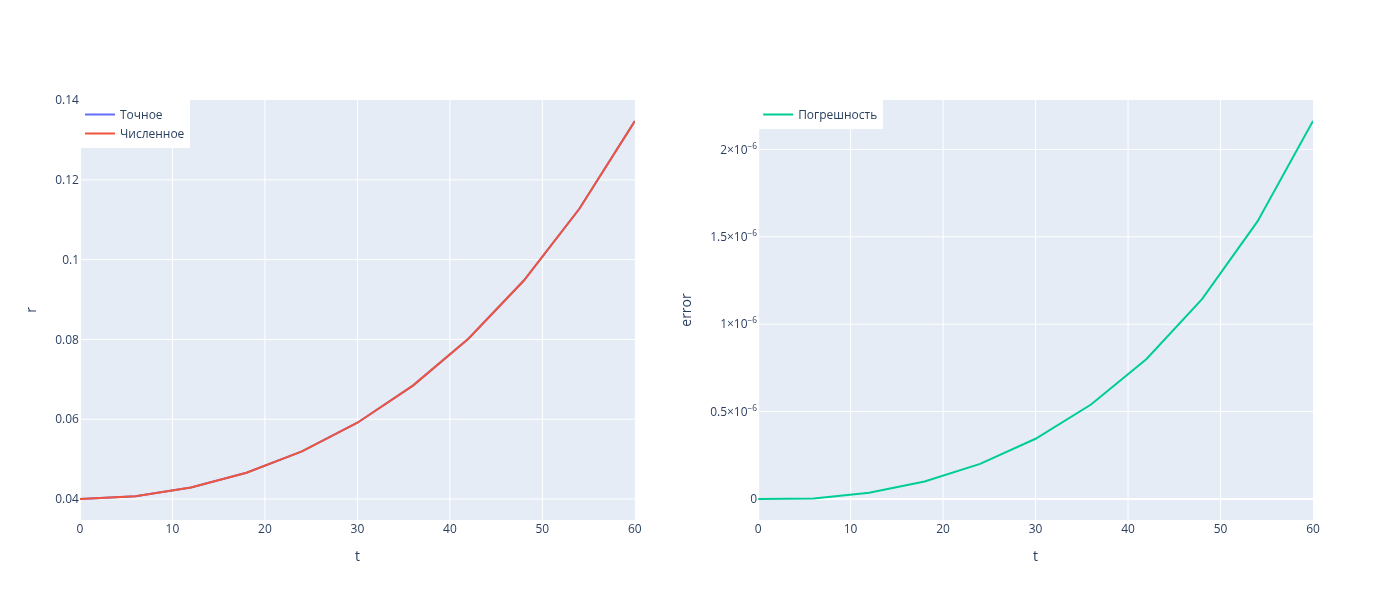
\includegraphics[width=\textwidth]{images/10.png}        
        \caption{Тестирование решения при $N = 10$}
        \label{n_10}
    \end{figure}

    \begin{figure}[H]
        \centering
        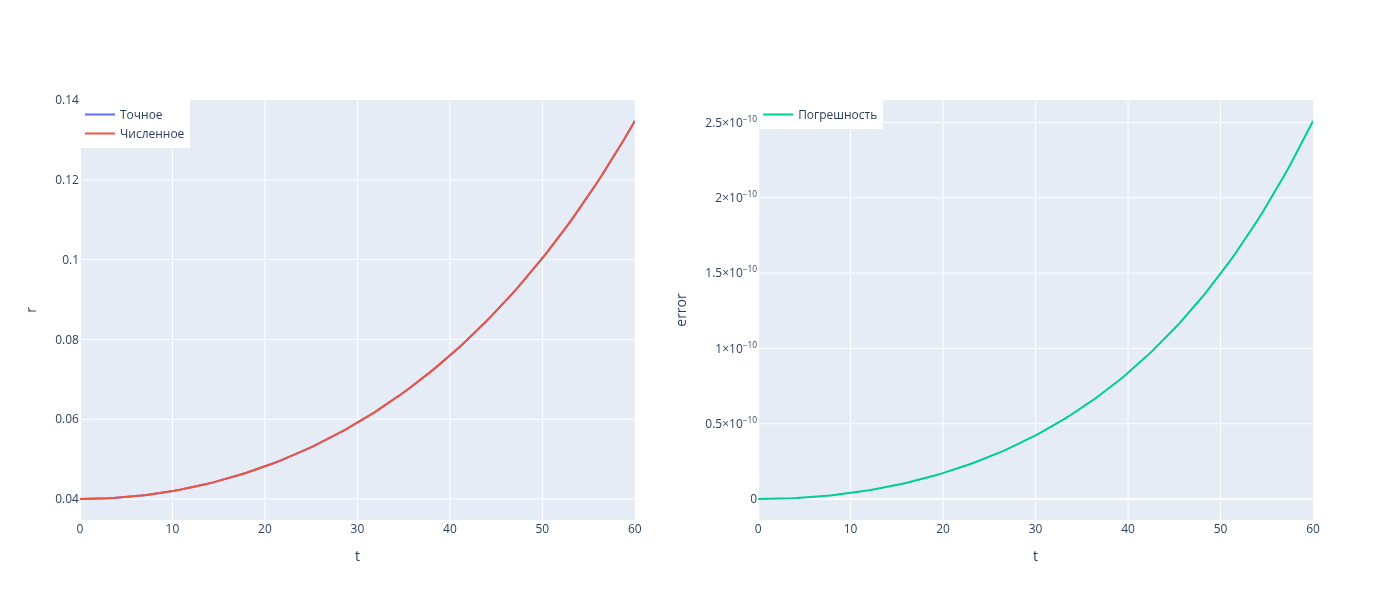
\includegraphics[width=\textwidth]{images/100.png}        
        \caption{Тестирование решения при $N = 100$}
        \label{n_100}
    \end{figure}

    \begin{figure}[H]
        \centering
        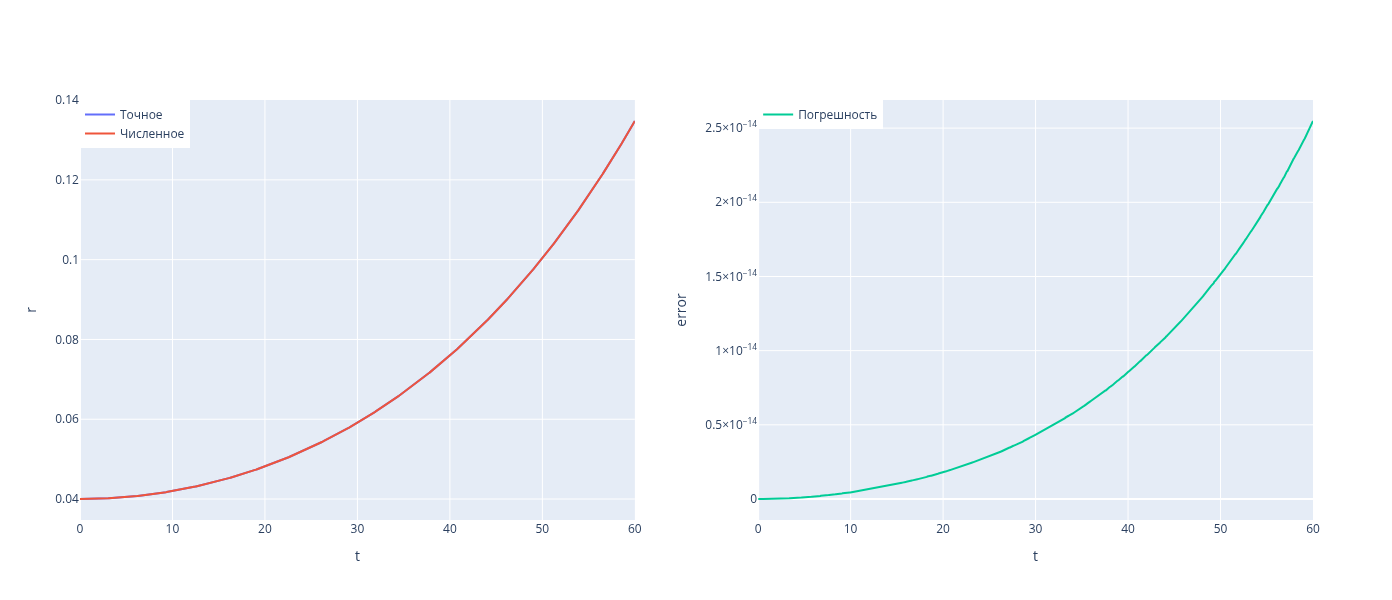
\includegraphics[width=\textwidth]{images/1000.png}        
        \caption{Тестирование решения при $N = 1000$}
        \label{n_1000}
    \end{figure}

    \section{Заключение}
    В ходе лабораторной работы была рассмотрена и решена задача на движение. 
    Сравнение численных и аналитических решений, приведённое на графиках (\cref{n_10}, \cref{n_100}, \cref{n_1000}), показало, что при увеличении числа узлов сетки численное решение всё точнее приближается к аналитическому. 
    Ответ был получен 0.135 м.
\end{document}